\newpage
\subsection*{(c)}
%
\begin{color}{AAUblue2}
%
Modificer \textsc{opg2-system.py} til et system hvor $\gamma$ kan ændres med udgangspunkt i at modelles første ser ud som følgende 
\begin{align}
\frac{dx_1}{dt} &= - \alpha x_1 x_2 - \gamma x_1, \\
\frac{dx_2}{dt} & = \alpha x_1 x_2 - \beta x_2 , \\
\frac{dx_3}{dt} & = \beta x_2 + \gamma x_1.
\end{align}
%
Beskriv hvad der sker med en ændring i gamma.  
%
\end{color}
\\\\
% 
Se \textsc{system-example-modi.py}. Implementeringerne er ved
\textbf{\textit{def f(t, x)}}, linje $60$.
\\\\
%
Introduceres en vaccine, hvor $\gamma$ beskriver, hvor hurtigt der kan vaccineres, vil dette have en effekt på smittespredningen.
Værdien gamma forøger dermed, hvor hurtigt befolkningen bliver immun uden at have været smittet. Jo højere værdi af gamma jo hurtigere bliver befolkningen immun.
Først ses på udgangspunktet, dog med vaccine.
Dette ses på figur \ref{fig:a1_b35_g5}.
%
\begin{figure}[!ht]
\centering
$
\begin{matrix}
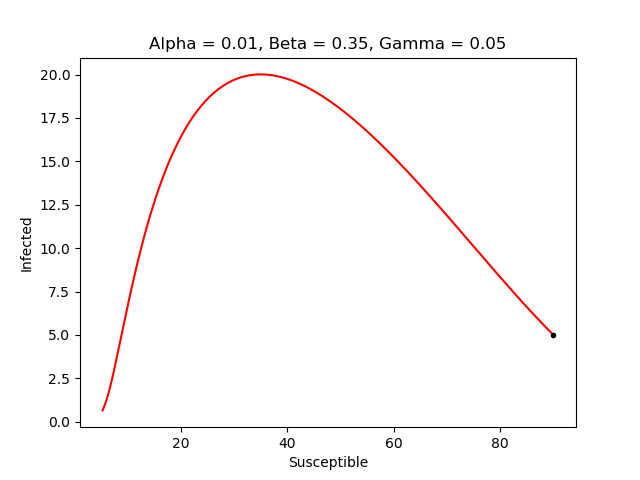
\includegraphics[scale=0.5]{fig/img/a1_b35_g5.png}&
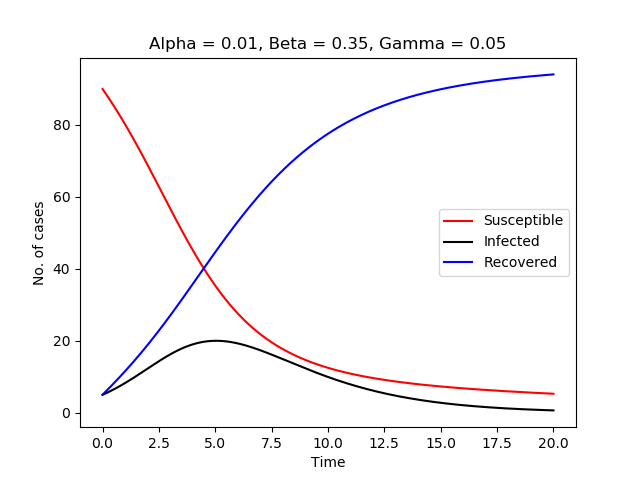
\includegraphics[scale=0.5]{fig/img/t_a1_b35_g5.png}
\end{matrix}
$
\caption{Smitten når $\alpha = 0.01$, $\beta = 0.35$ og $\gamma = 0.05$.}
\label{fig:a1_b35_g5}
\end{figure}
\\\\
%
Her ses det, at vaccinen ikke har effekt på hvornår smitten topper, men reducere toppen.
Naturligvis øger det også raten hvormed folk bliver immune.
%
\begin{figure}[!ht]
\centering
$
\begin{matrix}
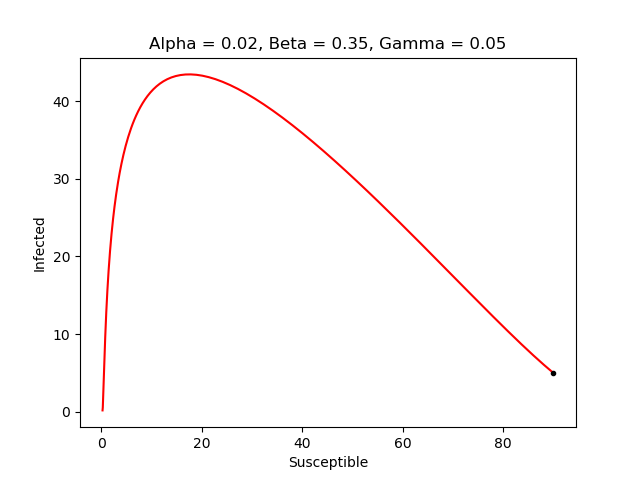
\includegraphics[scale=0.5]{fig/img/a2_b35_g5.png}&
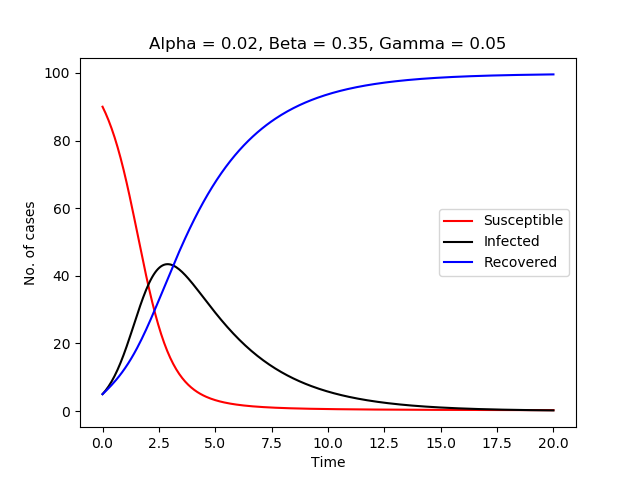
\includegraphics[scale=0.5]{fig/img/t_a2_b35_g5.png}
\end{matrix}
$
\caption{Smitten når $\alpha = 0.02$, $\beta = 0.35$ og $\gamma = 0.05$.}
\label{fig:a2_b35_g5}
\end{figure}
\\\\
%
Det samme lader til at være tilfældet selv når $\alpha$ er blevet fordoblet, hvilket kan ses på figur \ref{fig:a2_b35_g5}.
Det kan ses på figur \ref{fig:a1_b7_g5}, at når $\beta$ er fordoblet og der er tilføjet en vaccine er der dog ikke en betydelig forskel i antallet af smittede, men tilgengæld flatliner antallet af immune ikke med samme rate.
%
\begin{figure}[!ht]
\centering
$
\begin{matrix}
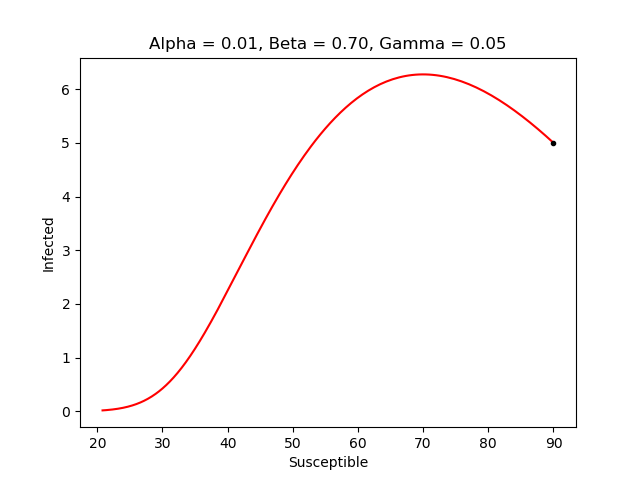
\includegraphics[scale=0.5]{fig/img/a1_b7_g5.png}&
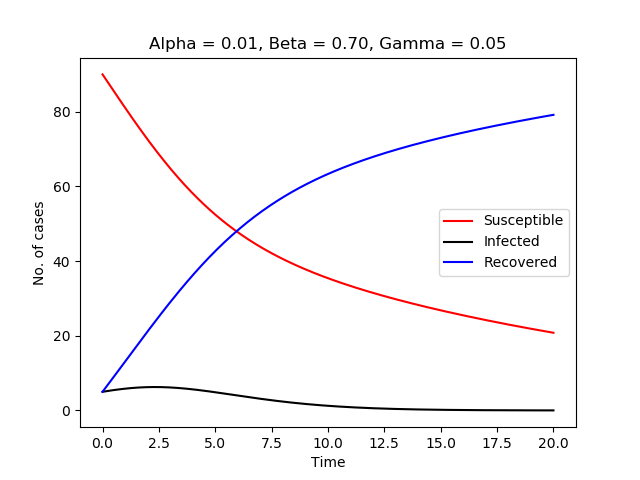
\includegraphics[scale=0.5]{fig/img/t_a1_b7_g5.png}
\end{matrix}
$
\caption{Smitten når $\alpha = 0.01$, $\beta = 0.7$ og $\gamma = 0.05$.}
\label{fig:a1_b7_g5}
\end{figure}
\\\\
%
Dermed falder det maksimale antal, der er smittet på en gang, og hvis gamma ikke er nul så er antallet, som bliver inficeret, lavere.